\documentclass[11pt]{article}

\usepackage[utf8]{inputenc}
\renewcommand{\baselinestretch}{1.25}
\usepackage{geometry, amsmath, amsthm, latexsym, amssymb, graphicx, amsfonts}


\title{Improving the optomechanics of a BAW resonator for quantum amplification within future gravitational wave detectors}
\author{Joseph Hocking\\\textbf{Supervisors:} Prof. C. Zhao, Prof. Ju Li}
\date{\today}

\begin{document}

\maketitle

\section{Introduction}
    \par
    Gravitational waves, ripples in the very fabric of space-time, were once thought to be the playground of theoretical physicists. A fun quirk falling out of Einstein's revolutionary theory of general relativity. That was until in September of 2015, when we first directly heard the rumblings of universe. A true testament to the hard work and utter dedication of over half a century of international collaboration. We are now on the cusp of a new era of astronomy, the era of gravitational wave detection. It was Feynman, in a conference in 1957, described the first gravitational wave detector (GWD) in a mock thought experiment. Imagine a rigid rod, with two beads freely sliding (with friction), as the gravity wave passes through the rod the rigidity of it does not allow it to move with the wave. However, the proper distance between the beads will move, and due to this some small amount of energy will be deposited within the system, energy from the wave itself. Thus a it was realised that, theoretically at the minimum, one could detect gravitational waves. It was quickly noted, however, that due to the incredible stiffness of space-time, there existed no such material that could resist the motion of the wave.
    \par
    The first experimental attempts at gravitational wave detections were through the use of \textit{Resonant Mass Antennas}. These, as shown in Figure \ref{pic:resonant_bar}, consist of a large bar precisely machine to have a resonant frequency matching that of expected gravitional wave sources. These achieved sensitivies on the order of $10^{-19}\varepsilon/\sqrt{Hz}$, chiefly through the use of advanced seismic isolation systems, cryogenic cooling, and materials with extreme mechanical Q-factors. There were some who claimed (and some who still do) that these incredible experimental system did detect gravitional waves, see \ref{ref:webber-detection}, but the consensus of the wider scientific community beleives that there simply were not sensitive enough.
    \begin{figure}
        \centering
        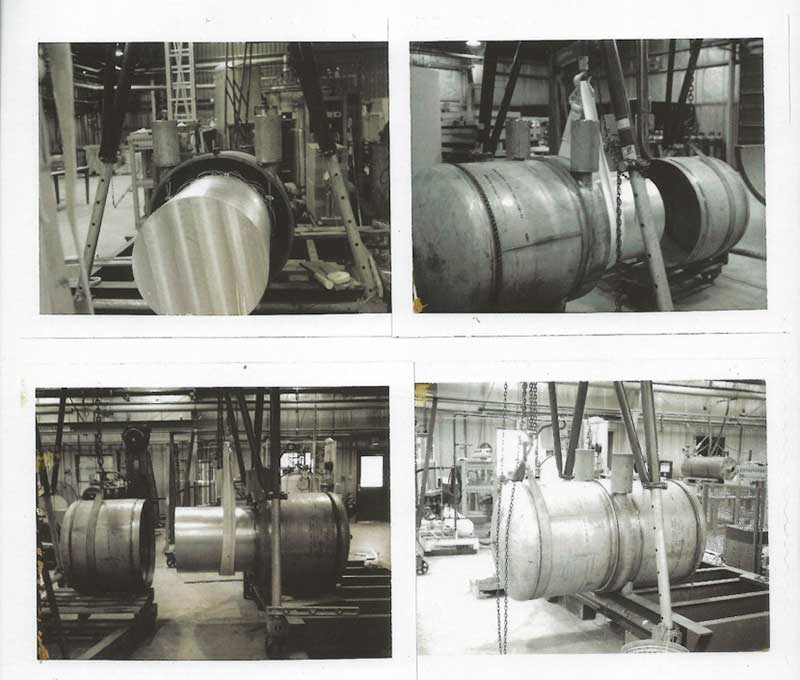
\includegraphics[width=0.5\textwidth]{img/weber-bar.jpg}
        \label{pic:resonant_bar}
    \end{figure}
    \par
    \textbf{WIP Section. Need clear explanation of GWDs}\\
    The next, and current, generation of GWDs came in the form of large laser-based interferometers. A high powered, usually 1064nm, laser is split down two arms, which have a mirror at their respective ends. The photons, upon returning destructively interfere at the output port. When a GW signal couples into the detector, one of the arms are slightly elongated, meaning that there ius no longer complete destructive interference and the signal is detected. This is a huge over simplification of the system but for the purposes of this proposal, it will suffice to illustrate the point. 

\section{The Noise Curve}
    \label{sec:noise-curve}
    For gravitational wave instrumentation, one of the most important figures is the interferometer noise curve, shown in ref{fig:noise-curve}. It is a measure of the minimum amplitude detectable by any given GWD, and can be seperated into several sources of noise. Within the low frequency regime, we become limited by the seismic motion of the ground the detector is situated upon. Then within the 10-20Hz range we begin to see the thermal noise of the suspension system spike. However, soon after that going all the way up to ~100Hz we are limited by radiation pressure noise. As the photons are reflected off the suspended mirrors, an imperceptible force is exterted, but due to the extreme laser powers and sensitivities, this small force is enough to push the mirror and produce noise within this frequency band. Beyond this, is where the research within this proposal focuses upon. In this high frequency band (1kHz) we are dominated by quantum shot noise. Due the Poisson counting statistics of the photons, the quantum shot noise is inversely proportional to the square root of the number of photons. Now normally when we have many photons hitting a photodetector, this variation is negligible, but at the high frequencies of the GW we no longer have the same power level, so this noise is dominates. 
    \subsection{Quantum Amplification}
    The crux of the question this research will attempt to answer is: "How can we fix this shot noise?". In order to answer this question, we must first understand why we lose power at the higher frequencies. This boils down to the nature of the arm resonators. These are powerful tools with interferometers, but they can be a double edged sword. Traditionally all resonators follow a \textit{gain-bandwidth relationship} where, for a given resonator design, we must maintain a fixed gain-bandwidth product, that is, if we wish to increase our gain, we must decrease our bandwidth. 
\end{document}